\documentclass[10pt]{article}
\usepackage[margin=0.8in]{geometry}
\usepackage[utf8]{inputenc}
\usepackage[T1]{fontenc}
\usepackage{graphicx}
\usepackage[export]{adjustbox}
\usepackage{amsmath}
\usepackage{amsfonts}
\usepackage{amssymb}
\usepackage[version=4]{mhchem}
\usepackage{stmaryrd}
\usepackage{bbold}
\usepackage{fixltx2e}
\usepackage{caption}
\usepackage{mathtools}
\usepackage[parfill]{parskip}
\usepackage{float}
\usepackage{amsmath}

\usepackage[framemethod=TikZ]{mdframed}
\colorlet{shadecolor}{orange!15}
\usepackage{xcolor}
\usepackage{amsthm}
\usepackage{framed}



\begin{document}



\title{Lecture 19: Overview of Robot Control}
\date{Nov. 17,  2023}
\author{Wanxin Jin}
\maketitle

\section{Overview of Robot Control}

The control of a robot manipulator is to determine the time sequence of control action (i.e., torques in each joint) to guarantee the execution of a specified task while satisfying the transient and steady-state error. In many robotics tasks, the task is specified usually in the operational space (such as end-effector motion and forces), whereas control (joint torque) is usually made in the joint space. There are two control schemes: joint space control and operational space control. In both schemes, the control architecture has closed loops. 


The joint space control scheme is shown in Fig. \ref{fig.joint_control}. First, manipulator inverse kinematics is solved to transform the specified end-effector motion  $\boldsymbol{x}_{d}$ to the corresponding joint motion $\boldsymbol{q}_{d}$ in the joint space. Then, a joint space control scheme is designed that allows the actual motion $\boldsymbol{q}$ to track $\boldsymbol{q}_{d}$. However, the controller does not \emph{directly} regulate the operational space  motion $\boldsymbol{x}_{e}$, thus, $\boldsymbol{x}_{e}$ is controlled in an open-loop fashion through the manipulator mechanical structure, which could have less accuracy due to the uncertainty of the structure (construction tolerance, lack of calibration, gear backlash, elasticity)...



\begin{figure}[H]
    \centering
    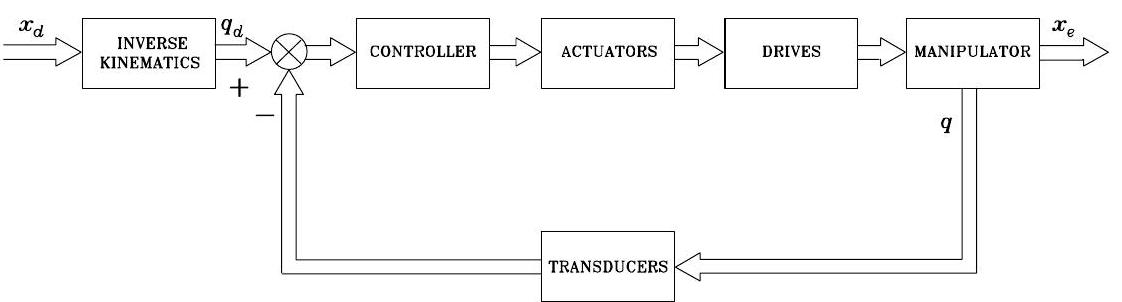
\includegraphics[max width=0.7\textwidth]{control/joint_control.jpg}
    \caption{Joint space control}
    \label{fig.joint_control}
\end{figure}


The operational space control  is shown in Fig. \ref{fig.operational_space_control}. In this control scheme,  inverse kinematics is now embedded into the feedback control loop, and the operational space  motion $\boldsymbol{x}_{e}$ is directly fed back to the controller. Thus, it addresses the drawbacks of joint space control. However, the control algorithm is typically of a greater  complexity, and measuring the operational space motion $\boldsymbol{x}_{e}$ is  challenging (such as typically using vision). 

\begin{figure}[H]
    \centering
    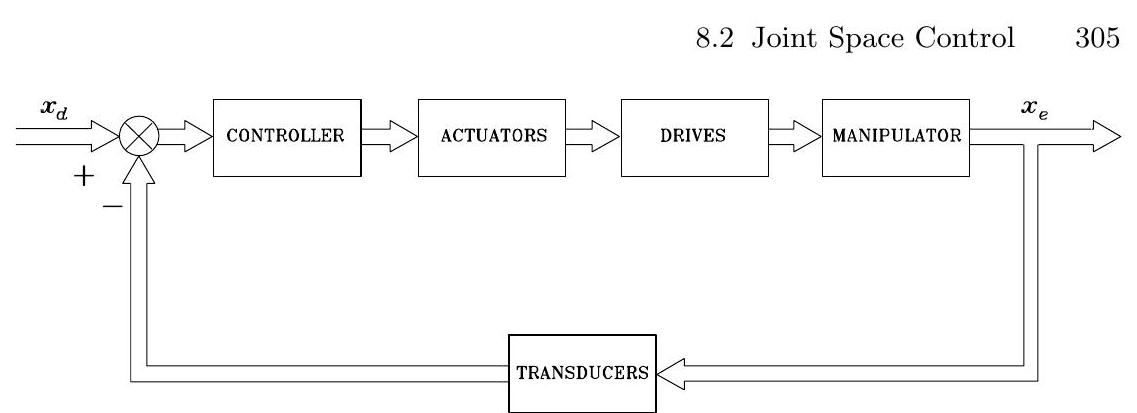
\includegraphics[max width=0.6\textwidth]{control/operational_space_control.jpg}
    \caption{Operational space control}
    \label{fig.operational_space_control}
\end{figure}





\section{Model of Acutuator}
According to the previous lecture, the equation of motion of a manipulator without external end-effector forces $\boldsymbol{h}_{e}$ and  static friction ($-\text{sign}(\boldsymbol{\dot{q}})$,  difficult to model accurately) is

$$
\boldsymbol{B}(\boldsymbol{q}) \ddot{\boldsymbol{q}}+\boldsymbol{C}(\boldsymbol{q}, \dot{\boldsymbol{q}}) \dot{\boldsymbol{q}}+\boldsymbol{F}_{v} \dot{\boldsymbol{q}}+\boldsymbol{g}(\boldsymbol{q})=\boldsymbol{\tau}
$$




\begin{figure}[H]
    \centering
    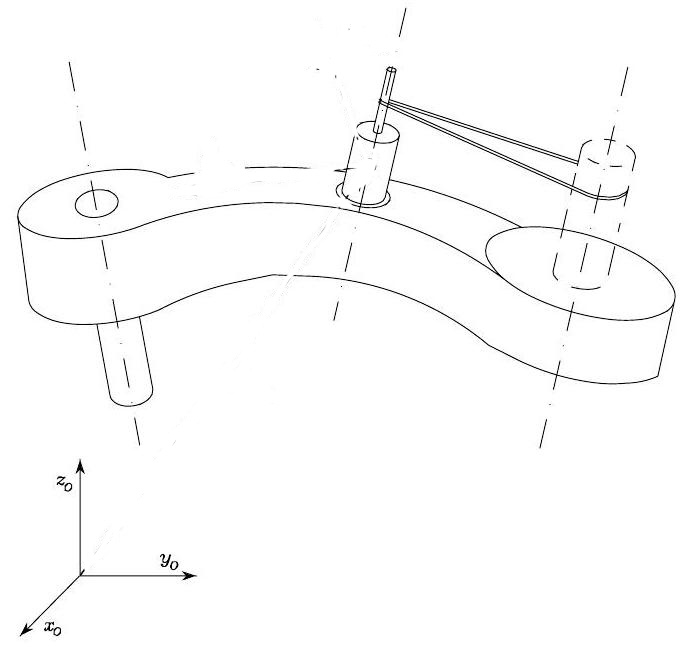
\includegraphics[max width=0.35\textwidth]{dynamics/motori_kinematics.jpg}
    \caption{Transmission between actuator (electric motor) and joint}
    \label{fig:enter-label}
\end{figure}

\subsection{Transmissions between Actuator and Joint}
 Let $\boldsymbol{q}_{m}$ denote the vector of joint actuator displacements (motor's rotor angle). The transmissions - assumed to be rigid and with no backlash - between the motor and joint motion is 

\begin{equation}\label{equ.transmission_model}
    \boldsymbol{K}_{r} \boldsymbol{q}=\boldsymbol{q}_{m}
\end{equation}

where $\boldsymbol{K}_{r}$ is a $(n \times n)$ diagonal matrix, typically much greater than identity. Let $\boldsymbol{\tau}_{m}$ denotes the vector of the actuator driving torques, based on principle of virtual work, one has the following  transmission between motor torque and joint torque:

\begin{equation}\label{equ.transmission_model2}
\boldsymbol{\tau}_{m}=\boldsymbol{K}_{r}^{-1} \boldsymbol{\tau}
\end{equation}

\subsection{Electric Motor (DC) Model}

\begin{equation}\label{equ.dc_model}
    \begin{aligned}
 \boldsymbol{\tau}_m& =\boldsymbol{K}_{t} \boldsymbol{i}_{a} \\
\boldsymbol{v}_{a} & =\boldsymbol{R}_{a} \boldsymbol{i}_{a}+\boldsymbol{K}_{v} \dot{\boldsymbol{q}}_{m} \\
\boldsymbol{v}_{a} & =\boldsymbol{G}_{v} \boldsymbol{v}_{c}
\end{aligned}
\end{equation}

Here, $\boldsymbol{K}_{t}$ is the torque constants;  $\boldsymbol{i}_{a}$ is the  armature currents; $ \boldsymbol{v}_{a}$ is the vector of armature voltages; $\boldsymbol{R}_{a}$ is the  armature resistances; $\boldsymbol{K}_{v}$ is the back EMF constants; $\boldsymbol{G}_{v}$ is the amplifiers; and $\boldsymbol{v}_{c}$ is the voltages of the servomotors.

Based on (\ref{equ.transmission_model}-\ref{equ.dc_model}), we have

\begin{equation}\label{equ.voltage_control}
    \boldsymbol{\tau}=\boldsymbol{K}_{r} \boldsymbol{K}_{t} \boldsymbol{R}_{a}^{-1}\left(\boldsymbol{G}_{v} \boldsymbol{v}_{c}-\boldsymbol{K}_{v} \boldsymbol{K}_{r} \dot{\boldsymbol{q}}\right) 
\end{equation}

The above equation unveils a relationship between the applied servomotor voltage $\boldsymbol{v}_c$, the generated joint torque $\boldsymbol{\tau}$, and the joint velocity $\boldsymbol{\dot{q}}$. The overall  diagram modeling DC motor and manipulator is shown in Fig. \ref{fig.voltage_control}.


\begin{figure}[H]
    \centering
    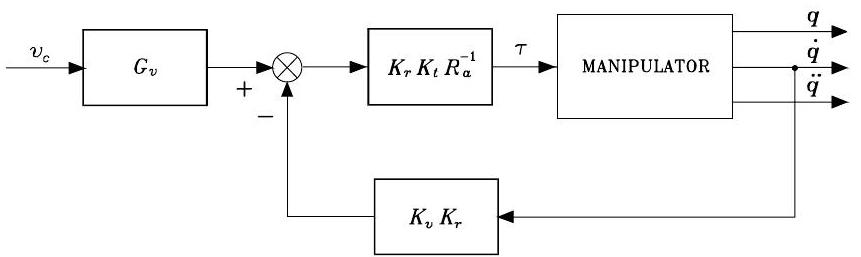
\includegraphics[max width=0.65\textwidth]{control/voltage_control.jpg}
    \caption{DC motor with manipulator}
    \label{fig.voltage_control}
\end{figure}


\section{Manipulator as an  Integrator (Approximately)!}

If the following assumptions hold for (\ref{equ.voltage_control}):

\begin{itemize}
  \item the elements of matrix $\boldsymbol{K}_{r}$, characterizing the transmissions, are much greater than unity;

  \item the elements of matrix $\boldsymbol{R}_{a}$ are very small, which is typical in the case of high-efficiency servomotors;

  \item the values of the joint torques $\boldsymbol{\tau}$ required for the execution of the desired motions are not too large;

\end{itemize}

then 

$$
\boldsymbol{G}_{v} \boldsymbol{v}_{c} \approx \boldsymbol{K}_{v} \boldsymbol{K}_{r} \dot{\boldsymbol{q}}
$$
and further 

\begin{equation}
    \boldsymbol{v}_{c} = \boldsymbol{G}_{v}^{-1} \boldsymbol{K}_{v} \boldsymbol{K}_{r} \dot{\boldsymbol{q}}
\end{equation}

The above equation says that, under the above-stated assumptions,  the whole system, i.e., DC motor plus manipulator, can be considered as a voltage-to-velocity system:  the joint velocity of a manipulator of is proportional to the voltage input to the servomotor. In other words, the manipulator plus the drive system can be considered as an integrator! 



The benefit of this system is that it is a decentralized control system (each joint can be controlled independently of the others): the velocity of the $i$-th joint depends only on the $i$-th control voltage, since the matrix $\boldsymbol{G}_{v}^{-1} \boldsymbol{K}_{v} \boldsymbol{K}_{r}$ is diagonal.  




\section{Torque-Controlled System (more general cases)}
If the assumption in the above section does not hold, the whole system, for example, when $\left(\boldsymbol{K}_{r}=\boldsymbol{I}\right)$, we do not have such a nice property of "manipulator as an integrator". In those cases,  we still have the following relation between the computed joint torque and armature current

\begin{equation}\label{equ.current_torque}
    \boldsymbol{K}_r^{-1}\boldsymbol{\tau}= \boldsymbol{\tau}_m =\boldsymbol{K}_{t} \boldsymbol{i}_{a}
\end{equation}

Thus, typically, we have a local feedback control system inside the motor to regulate the armature current $\boldsymbol{i}_a$. This local control system will establish the following relationship between the voltage of the servomotor and the current:

\begin{equation}\label{equ.voltage_current}
    \boldsymbol{i}_{a}=\boldsymbol{G}_{i} \boldsymbol{v}_{c}
\end{equation}

Therefore, based on (\ref{equ.current_torque}) and (\ref{equ.voltage_control}), we have


\begin{equation}\label{equ.voltage_current}
    \boldsymbol{\tau}=\boldsymbol{K}_r\boldsymbol{K}_{t}\boldsymbol{G}_{i} \boldsymbol{v}_{c}
\end{equation}

The above equation says that, in the general case,  the whole system, i.e., DC motor plus manipulator, can be considered as a voltage-to-torque system: you can directly regulate  the joint torque of a manipulator by regulating the voltage to the servomotor. 



\end{document}